%\section{Event Reconstruction and Analysis} 

The \minerva\ detector records the energy and time of energy depositions (hits) in each scintillator strip.  Hits are first grouped in time and then clusters of energy are formed by spatially grouping the hits in each scintillator plane.  Clusters with energy $>\unit[1]{MeV}$ are then matched among the three views to create a track. The most upstream cluster on the muon track establishes the event vertex. We identify a $\mu^+$ by matching a track that exits the back of \minerva with a positively charged track entering the front of \minos. The per plane track resolution is 2.7~mm and the angular resolution of the
muon track is better than 10~mrad~\cite{minerva_nim}.  
 The event vertex is restricted to be within the central 110 planes of the scintillator tracking region and no closer than \unit[22]{cm} to any edge of the planes. These requirements define a region with a mass of \unit[5.57]{metric tons}.

%The event vertex is restricted to a hexagon of apothem 85~cm centered  on the \minerva detector and must be within the central 110 planes  of the fully active detector.  These requirements define a region  with a mass of 5.57~tons.

The times of the tracked hits are used to determine the interaction time.  
Other untracked clusters up to \unit[20]{ns} before and 
\unit[35]{ns} after that time are associated with the event.  The energy of the 
recoil system  is calculated from all clusters not associated with the muon
track or located within the vertex region.
Events with two or more isolated groups of
spatially contiguous clusters 
%of recoil energy 
are rejected as likely to be due to 
inelastic backgrounds.

Event pile-up causes a decrease in the muon track reconstruction efficiency. We studied this in both \minerva and \minos by projecting tracks found in one of the detectors to the other and measuring the misreconstruction rate. This resulted in a -7.8\% (-4.6\%) correction to the simulated efficiency for muons below (above) 3 GeV/c.

Estimation of the initial neutrino energy ($E_\nu$) and 
four-momentum transfer squared ($Q^2$) of the
interaction assumes an initial state nucleon at rest with a constant
binding energy, $E_b$, which we set to $\unit[+30]{MeV}$ based on
electron scattering data~\cite{Moniz:1971mt,VanOrden:1980tg} and estimates of Coulomb and asymmetry (Pauli) energy effects from the semi-empirical 
mass formula for nuclei~\cite{Katori:2008zz}. 
Under this quasi-elastic hypothesis,
denoted by $QE$, 
\begin{eqnarray}
E_\nu^{QE} &=& \frac{m^2_n - (m_p-E_b)^2-m_\mu^2+2(m_p-E_b)E_\mu}{2(m_p-E_b-E_\mu+p_\mu \cos\theta_\mu)} \label{eq:enudef} \\
%{\rm\textstyle and}~
Q^2_{QE} &=& 2E_\nu^{QE}(E_\mu-p_\mu \cos\theta_\mu ) - m_\mu^2, \label{eq:q2def}
\end{eqnarray}
where $E_\mu$ and $p_\mu$ are the muon energy and momentum, $\theta_\mu$ is the muon angle
with respect to the beam and $m_n$, $m_p$ and $m_\mu$ are the masses
of the neutron, proton and muon, respectively.

Figure~\ref{fig:recoil_fits} shows the reconstructed data compared 
to neutrino interactions simulated 
using the GENIE 2.6.2 neutrino event generator~\cite{Andreopoulos201087}.  
For quasi-elastic interactions,  the cross-section is given by the 
Llewellyn Smith formalism~\cite{LlewellynSmith:1971zm}.  
Vector form factors come from fits 
to electron scattering data~\cite{Bradford:2006yz}; 
the axial form factor used is a dipole with an axial mass 
($M_A$) of 0.99~GeV$/$c$^2$, consistent with 
deuterium measurements~\cite{Bodek:2007vi,Kuzmin:2007kr}; and
sub-leading form factors are assumed from PCAC or exact G-parity
symmetry~\cite{Day:2012gb}.  The nuclear model is the relativistic
Fermi gas (RFG) 
with a Fermi momentum of $221$~MeV$/$c and an extension to higher 
nucleon momenta to account for short-range 
correlations~\cite{Bodek:1980ar,Bodek:1981wr}.
Inelastic reactions with a low invariant mass hadronic final state are based on a tuned model of discrete
baryon resonance production~\cite{Rein:1980wg}, and the transition to deep inelastic scattering is simulated using the Bodek-Yang
model~\cite{Bodek:2004pc}.   Final state interactions, where hadrons
interact within the target nucleus, are modeled using the INTRANUKE
package~\cite{Andreopoulos201087}.

\begin{figure}[tp]
\centering
\ifnum\PRLsupp=0
  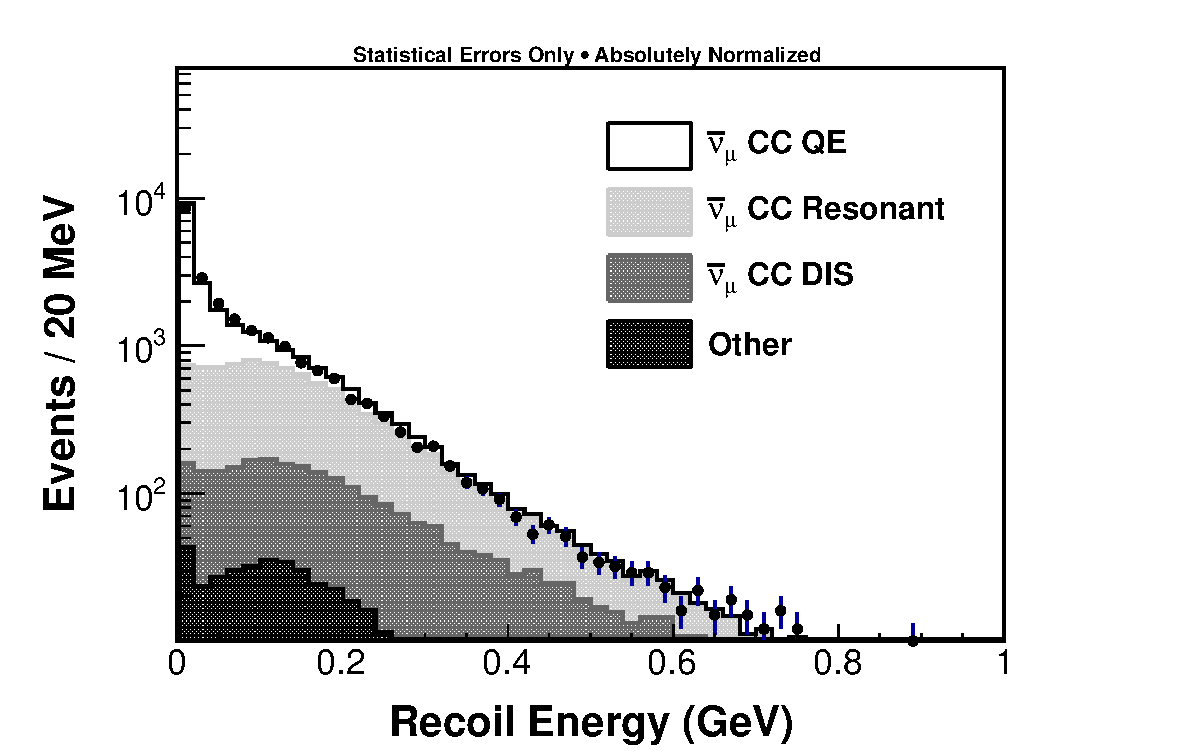
\includegraphics[width=\columnwidth]{figures/Figure1_anu} 
\else
  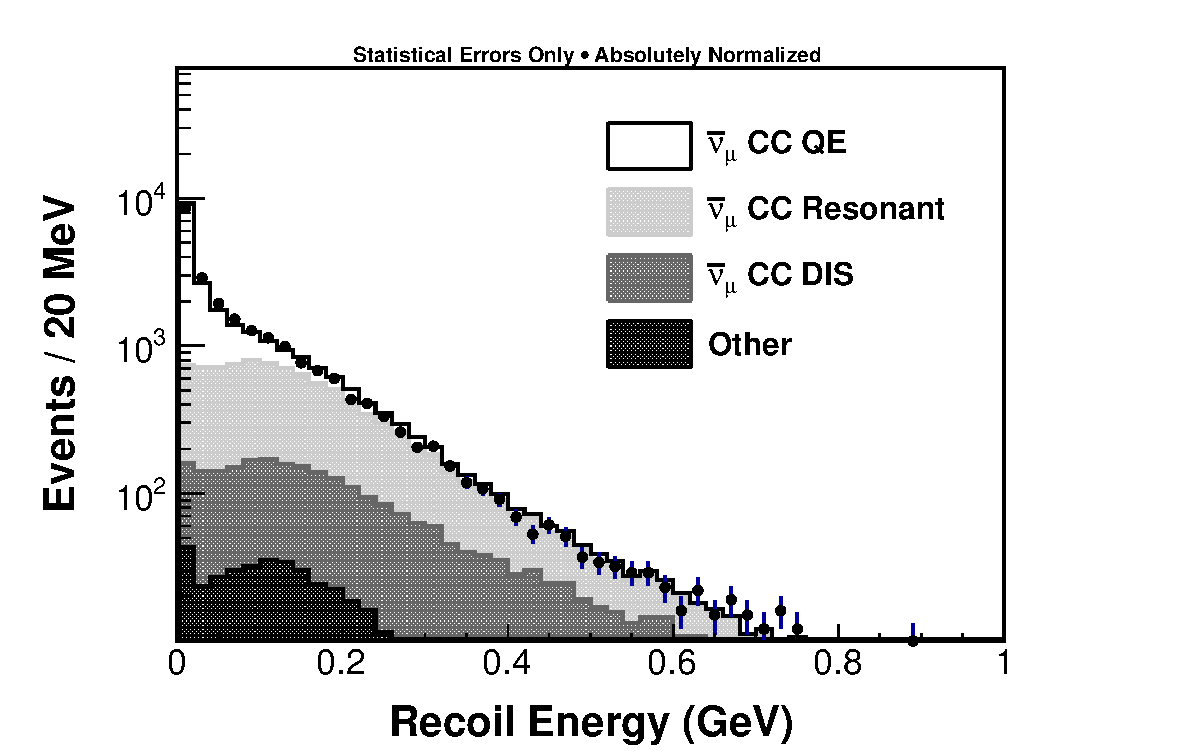
\includegraphics[width=0.8\columnwidth]{figures/Figure1_anu} 
\fi
\caption{The measured recoil energy distribution (solid circles) and the predicted composition of signal and background. Backgrounds from baryon resonance production (light grey), continuum/deep-inelastic scattering (dark grey), and other sources (black),such as coherent pion production, are shown.  The fraction of signal in this sample, before requiring low recoil energy, is $0.58$.}
\label{fig:recoil_fits}
\end{figure}

\begin{figure}[tp]
\centering
\ifnum\PRLsupp=0
  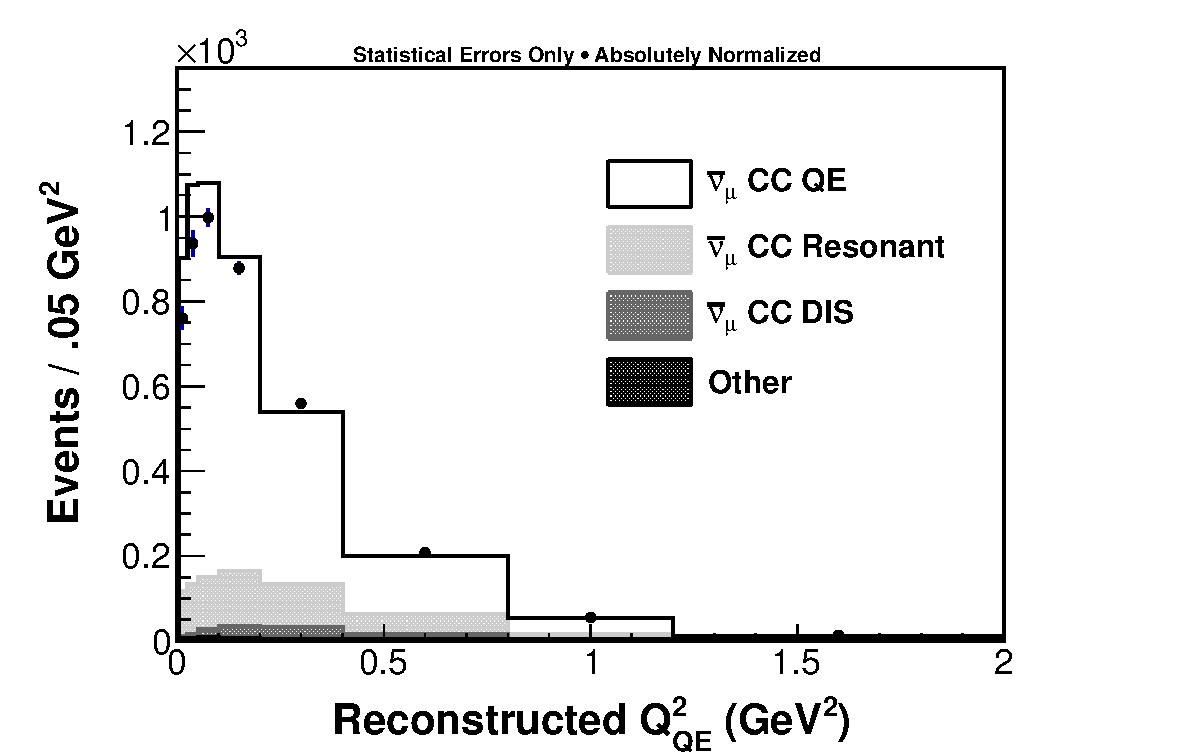
\includegraphics[width=\columnwidth]{figures/Figure2_anu} 
\else
  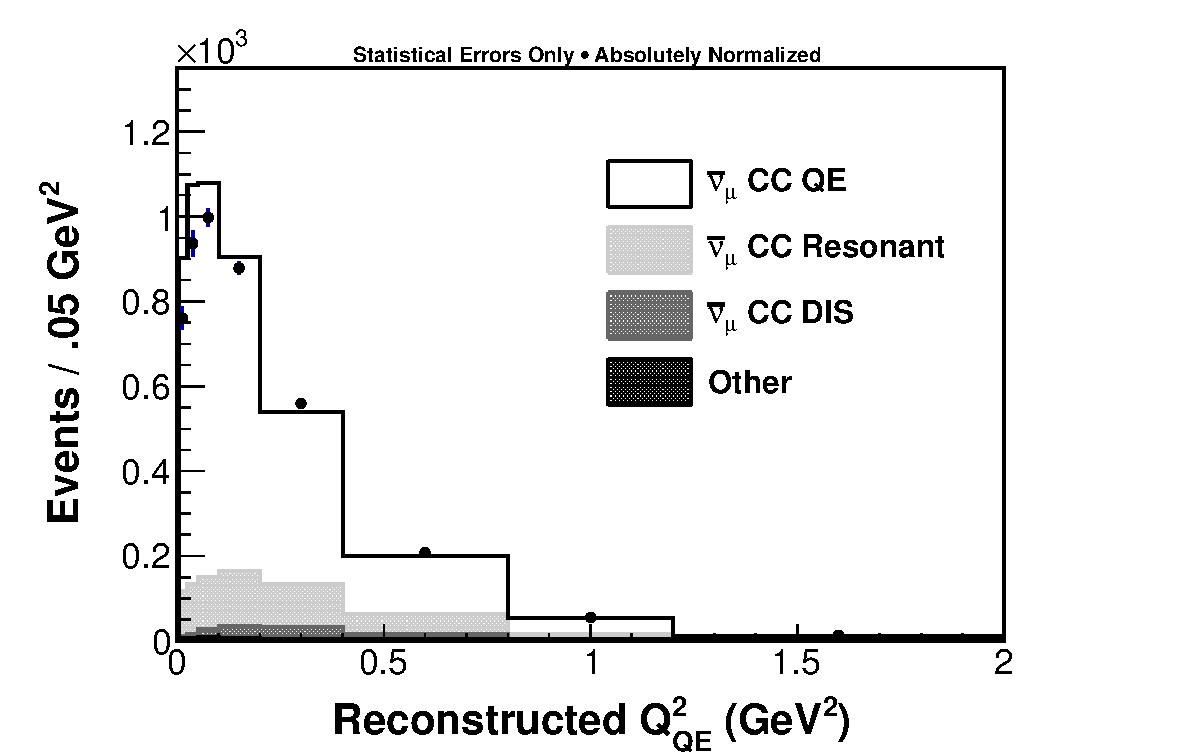
\includegraphics[width=0.7\columnwidth]{figures/Figure2_anu} 
\fi
\caption{\label{fig:qsq} The measured $Q^2_{QE}$ distribution before background subtraction and corrections for detector resolutions and acceptance.  The fraction of signal in this sample is $0.77$, and 54\% of signal events in our fiducial volume pass all selections.}
\end{figure}

Figure~\ref{fig:recoil_fits} shows evidence of quasi-elastic interactions in the
peak of events at low recoil energy. A significant background of 
inelastic events still exists, primarily from baryon resonance 
production and decay where the final state pion is not identified.  To reduce this 
background we make a $Q^2_{QE}$ dependent selection of low recoil-energy events\footnote{{T}he precise selection is $E_\text{recoil} < 0.03+0.3\times Q^2_{QE}$(GeV$^2/$c$^2$). The $Q^2_{QE}$ dependence improves the signal efficiency for higher $Q^2_{QE}$.}.  We also require $E_\nu^{QE} < \unit[10]{GeV}$ to limit uncertainties due to the neutrino flux. Figure~\ref{fig:qsq} shows the $Q^2_{QE}$ 
distribution of the remaining 16,467 events in the data compared with the simulation. 

% MAK, the 1\% background sentence doesn't fit very well here and I'm not sure we need it
% The $\mu^-$ background predicted by the simulation is less than 1\%.

%At this point the signal efficiency is estimated at xx\% and the
%purity of the sample is estimated at yy\% .



